Электрический ток представляет собой направленный перенос зарядов. Микрочастицы,
осуществляющие этот перенос, называют \term{носителями тока}. В конце
XIX века в опытах Дж.~Дж.~Томсона с <<катодными лучами>> были открыты
элементарные носители заряда~--- \term{электроны}. Вскоре были проведены
первые измерения величины элементарного заряда: Р.~Милликен
в опытах в 1908--1916 годов измерял заряд микроскопических капелек масла,
помещённых во внешнее электрическое поле. Идея этих опытов проста:
если элементарный заряд действительно существует, то величина заряда~$q$
любого тела может принимать только дискретную последовательность значений.
Сравнивая между собой заряды капель, можно убедиться в том, что все они
кратны одному и тому же числу~--- элементарному заряду~$e$:
\begin{equation*}
    q = 0,\,\pm e,\,\pm2e,\,\pm3e,\, \ldots
\end{equation*}
Величина заряда оказалась равной
\[
e\approx1,6\cdot 10^{-19}~Кл\qquad (e=4,8\cdot 10^{-10}~ед.~СГС).
\]
Сразу после этого по отклонению <<катодных лучей>> в магнитном поле была
измерена и масса электрона $m_e\approx 9,1\cdot 10^{-31}$~кг.

Свободные электроны могут являться носителями тока в свободном от вещества
пространстве (ток в вакуумном диоде, ионный пучок в масс-спектрометре, и
т.\,д.). Понятие носители тока \important{в веществе} уже не является таким
наглядным. Хотя в металлах и полупроводниках перенос заряда происходит
вследствие перемещения всё тех же электронов, их движение уже не является
движением свободных частиц, как в вакууме. Электроны движутся в сильном
периодическом поле, образованном ионами кристаллической решётки, и
взаимодействуют между собой, причём это движение и это взаимодействие
подчиняются законам квантовой механики. По этим законам получается, что перенос
заряда можно по-прежнему интерпретировать как движение свободных заряженных
частиц (точнее, \important{квази}частиц), но масса этих частиц, называемая
\term{эффективной массой}, \important{не совпадает с массой свободного
электрона}: $m_{e}^{эфф}\ne m_e$. Более того, полупроводники и некоторые металлы
ведут себя так, будто вместо электронов ток в них переносят некоторые
положительные частицы~--- так называемые \term{дырки}. Дырки подобны
элементарным частицам позитронам~--- в электрических и магнитных полях они
движутся как положительно заряженные частицы с элементарным зарядом $q_p=+e$, но
с некоторой эффективной массой $m_p^{эфф}\ne m_e$.

Таким образом, в физике металлов и полупроводников в качестве носителей тока
рассматривают \term{квазичастицы},
\important{не существующие отдельно от рассматриваемого вещества}.
Заряд этих носителей численно точно равен заряду электрона и может быть как
отрицательным, так и положительным. В~первом случае они по-прежнему называются
\term{электронами} (хотя их масса не равна $m_e$),
во втором~--- \term{дырками}. В~полупроводниках присутствуют оба типа этих
носителей, в большинстве металлов имеются только отрицательные носители.


\introsection{Движение заряженных частиц во внешних полях}

Рассмотрим два простейших примера движения свободных зарядов в вакууме под
действием электрического и магнитного полей. Такие условия движения реализуются,
например, в электронных вакуумных приборах, таких, как электронно-лучевая
трубка или вакуумный диод.


\introsubsection{Движение в однородном магнитном поле}

Как известно, на заряд~$q$, движущийся со скоростью~$\vec{v}$ в магнитном поле
$\vec{B}$, действует \term{сила Лоренца}:
\begin{equation*}
    \eqmark{3.1}
    \vec{F}=q{\vec{v}}\times{\vec{B}}.
\end{equation*}

Рассмотрим точечный заряд, движущийся с некоторой скоростью~$\vec{v}$ в
однородном магнитном поле $\vec{B}=\const$, перпендикулярном направлению
скорости, $\vec{v}\perp \vec{B}$. На движущийся электрон действует сила
$F=qvB$. Эта сила перпендикулярна скорости движения, и поэтому не изменяет её
абсолютной величины. Траектория движения заряда в этом случае является
\important{окружностью}. Сила~$F$ является центростремительной, поэтому
\[
m\frac{v^2}{r}=evB.
\]
Отсюда находим радиус~$r$ траектории, называемый \term{ларморовским радиусом}:
\begin{equation}
    \eqmark{3.2}
    r_B =\frac{m v}{qB}= \frac{v}{\omega_B},
\end{equation}
где
\begin{equation}
    \eqmark{omega-B}
    \omega_B=\frac{qB}{m}
\end{equation}
--- угловая скорость циклотронного вращения (\term{циклотронная частота}).
Такое движение частицы называется \term{циклотронным вращением}.

Заметим, что циклотронная частота не зависит от энергии частицы, так
что в однородном магнитном поле все частицы одного сорта вращаются с
\important{одинаковой} частотой. Частицы с разными знаками заряда вращаются в
противоположные стороны.

Пусть теперь заряд движется под некоторым углом~$\alpha$ к вектору
индукции~$\vec{B}$. Скорость заряда~$\vec{v}$ можно разложить
на две составляющие, перпендикулярную и параллельную магнитному полю:
\begin{equation*}
    v_{\perp}=v\sin\alpha,\qquad v_{\parallel}=v\cos\alpha.
\end{equation*}
Параллельная составляющая не вызывает появление силы Лоренца, поэтому
проекция траектории на плоскость, перпендикулярную~$\vec{B}$,
по-прежнему представляет собой окружность с ларморовским радиусом,
определяемым поперечной составляющей скорости:
\begin{equation}
    \eqmark{3.4}
    r_B =\frac{m v_{\perp}}{qB}.
\end{equation}
В~направлении поля~$\vec{B}$ на заряд не действуют никакие силы,
следовательно, в этом направлении он движется равномерно со скоростью
$v_{\parallel}=\const$. Таким образом, траектория заряда представляет собой
\important{винтовую линию}.

\todo[inline,author=Popov]{Сделать картинку}

Наконец, если включить электрическое поле, \important{параллельное}
магнитному $\vec{E}\parallel\vec{B}$, то частица будет двигаться с ускорением
вдоль оси $\vec{E}$. На её циклотронное движение в плоскости, перпендикулярной
$\vec{E}$, это никак не повлияет.

\introsubsection{Дрейф в скрещенных электрическом и магнитном полях}

Рассмотрим движение заряда $q$ во взаимно перпендикулярных однородных
электрическом и магнитном полях $\vec{E}\perp\vec{B}$
(рис.~\figref{Crossed fields}).

Уравнение движения заряда в таком случае имеет вид
\[
m\dot{\vec{v}} = q\vec{E} + q \vec{v}\times \vec{B}.
\]
Направим ось $z$ вдоль~$\vec{B}$, а ось $y$~--- вдоль~$\vec{E}$.
Тогда, разделив на $m$, получим
\begin{equation}
    \eqmark{3.9}
    \begin{aligned}
        \dot{v}_x&=\omega_B v_y,\\
        \dot{v}_y&=\tfrac{q}{m}E-\omega_B v_x,\\
        \dot{v}_z&=0,
\end{aligned}
\end{equation}
где $\omega_B = qB/m$~--- циклотронная частота.

Зададим нулевые начальные условия:
\[x(0)=y(0)=0,\quad v_x(0)=v_y(0)=0.\]
Непосредственной подстановкой несложно убедиться в том, что решением системы
дифференциальных уравнений является \important{циклоида}.
В параметрической форме:
\begin{equation}
    \eqmark{3.11}
    x = Vt - R\sin\omega_B t,\qquad y = r(1-\cos\omega_B t),
\end{equation}
где $V=E/B$, $r=V/\omega_B$.

Таким образом, движение в скрещенных электрическом и магнитном полях
$\vec{E}\perp \vec{B}$ представляет собой наложение
а) вращения с циклотронной частотой~$\omega_B$ в плоскости,
перпендикулярной~$\vec{B}$, и б) смещения (\term{дрейфа}) центра ларморовской
окружности с постоянной скоростью
\begin{equation}
    V_{др} = \frac{E}{B}
\end{equation}
в направлении, перпендикулярном~$\vec{E}$ и~$\vec{B}$. Это явление
называют \term{дрейфом в скрещенных полях}.

Примечательно, что
скорость и направления дрейфа \important{не зависят от свойств частицы}:
ни от её массы, ни от величины или знака заряда.

\todo[inline,author=Popov]{Сделать картинку}

\paragraph{Альтернативный вывод.}
Тот же результат можно получить другим способом. Воспользуемся
формулой для преобразования полей при смене системы отсчёта. В нерелятивистском
случае:
\[
\vec{E}' = \vec{E} + \vec{V}\times \vec{B},\qquad \vec{B}'=\vec{B}.
\]
Первое соотношение есть ни что иное как условие инвариантности силы
Лоренца при смене системы отсчёта. Подберём скорость~$\vec{V}$ так, чтобы
электрическое поле $\vec{E}'$ в системе, движущейся с этой скоростью, обратилось
в нуль:
\[
 0 = \vec{E} + \vec{V}\times \vec{B}.
\]
Поскольку $\vec{E}\perp \vec{B}$, решение этого уравнения однозначно:
\begin{equation}
    \vec{V}_{др} = \frac{\vec{E}\times \vec{B}}{B^2}.
\end{equation}
При переходе в эту систему останется только магнитное поле, поэтому
траектория частицы будет \important{ларморовской} (\important{циклотронной})
\important{окружностью}. Движение же самой системы будет как раз соответствовать
\important{дрейфу} центра этой окружности поперёк~$\vec{E}$ и~$\vec{B}$.

\begin{lab:note}
Заметим, что наши результаты получены в \important{нерелятивистском}
приближении. Для их применимости необходимо выполнение условия $V_{др}\ll c$,
то есть электрическое поле должно быть мало по сравнению с магнитным: $E\ll cB$.
Если $E>cB$, то во-первых, корректное рассмотрение возможно только с учётом
релятивизма, а во-вторых, движение не будет иметь характер дрейфа,
\end{lab:note}


\introsection{Электрический ток в вакуумном диоде}

Вакуумный диод --- это откачанный до высокого вакуума сосуд,
в котором разность потенциалов подана расположенные в нём электроды:
катод и анод. Электрический ток в диоде представляет собой упорядоченное
движение
свободных электронов, испускаемых катодом.  При этом электроны практически не
испытывают сопротивления своему движению, в отличие от обычного проводника.
Еще одной характерной особенностью такой системы является наличие
пространственного заряда. Как следствие, для вакуумного диода не применим закон
Ома.

Явление испускания электронов поверхностью твёрдого тела или жидкости называется
\term{электронной эмиссией}. Для удаления электрона из твёрдого вещества в
вакуум необходимо совершить работу, называемую \term{работой выхода} $A_{вых}$
(у чистых металлов $A_{вых}\sim 1\;эВ$).
Один из механизмов эмиссии --- испускание электронов с поверхности сильно
нагретых тел (\term{термоэлектронная эмиссия}). Работа выхода при этом
совершается за счёт кинетической энергии электронов, которой они обладают
внутри тела.

Если создать электрическое поле вне металла, оно будет увлекать вышедшие
электроны и через вакуум потечёт электрический ток.
С повышением температуры поверхности экспоненциально быстро растёт доля частиц,
способных преодолеть потенциальный барьер $A_{вых}$,
и следовательно, растёт интенсивность эмиссии электронов. Это приводит к тому,
что
в пространстве диода~--- особенно вблизи катода~--- накапливается отрицательный
объёмный заряд, экранирующий внешнее поле. Из-за этого результирующий ток
в диоде оказывается значительно меньше тока, который может обеспечить
эмиссия с катода. Такой режим работы диода называют \term{режимом объёмного
заряда}.

При достижении определённого напряжения дальнейшее нарастание тока практически
прекращается~--- ток достигает предельного значения $I_{нас}$, называемого
\term{током насыщения}. Это обусловлено ограниченностью эмиссионной способности
катода~--- величина тока насыщения определяется количеством электронов,
которое способно выйти из поверхности катода в единицу времени.

\paragraph{<<Закон 3/2>> для вакуумного диода.}
Рассмотрим режим объёмного заряда в простейшем случае \important{плоского}
диода.
Его электроды представимы в виде двух параллельных плоскостей,
между которыми задано напряжение $V$. Расстояние~$d$ между электродами много
меньше их площади. Направим ось~$x$ перпендикулярно к поверхности катода
в сторону анода, совместив начало координат с катодом. Задача
становится одномерной: все величины являются функциями только координаты~$x$.

Запишем для электрического поля \important{теорему Гаусса} в дифференциальной
форме:
\[
\frac{dE}{dx} = \frac{\rho}{\varepsilon_0},
\]
где~$\rho(x)$~--- \important{плотность электрического заряда}. По определению
потенциала электростатического поля имеем
\[
E = -\frac{d\varphi}{dx}.
\]
Отсюда находим, что $\varphi(x)$ удовлетворяет уравнению
\begin{equation}
    \eqmark{3.14}
    \frac{d^2\varphi}{dx^2}=-\frac{\rho}{\varepsilon_0}.
\end{equation}
Это частный (одномерный) случай \term{уравнения Пуассона}.

\important{Плотность тока} в диоде равна $j=\rho v$, где $v$~--- скорость
электронов. В стационаре заряд нигде не накапливается, поэтому плотность тока
всюду одинакова: $j=\const$. Из закона сохранения энергии имеем:
\begin{equation*}
    \frac{mv^2}{2}=e\varphi.
\end{equation*}
Здесь мы выбрали начало отсчёта потенциала на катоде, а также
\important{пренебрегли начальными (тепловыми) скоростями},
с которыми вылетают электроны с поверхности катода. Это можно сделать, если
приложенное напряжение достаточно велико: $eV\gg mv_0^2/2$.

Исключив из полученных соотношений плотность электронов~$\rho$ и скорость~$v$,
приходим к уравнению
\begin{equation}
    \eqmark{3.15}
    \frac{d^2\varphi}{dx^2}=\sqrt{\frac{m}{2e\varphi}} \frac{j}{\varepsilon_0}
\end{equation}
с граничными условиями
\begin{equation*}
 \varphi(0)=0,\qquad \varphi(d)=V.
\end{equation*}

Для однозначного решения этого дифференциального уравнения необходимо ещё одно
граничное условие. В общем случае это должна быть связь между плотностью
тока~$j$ и электрическим полем на поверхности катода
$E_0 = -\left.\frac{d\varphi}{dx}\right|_{x=0}$,
которую однако теоретически установить затруднительно.
Учтём, что в режиме объёмного заряда количество электронов, способных покинуть
катод из-за его нагрева, значительно превосходит ток в диоде.
Следовательно, \important{эмиссионная способность катода практически не
ограничена}. Поэтому, чтобы плотность тока оставалась конечной,
напряжённость электрического поля внутри катода должна быть мала: $E_0\to 0$.
Таким образом, получаем дополнительное граничное условие в виде
\begin{equation*}
    \left.\frac{d\varphi}{dx}\right|_{x = 0}=0.
\end{equation*}

Прямой подстановкой можно проверить, что решением \eqref{3.15},
удовлетворяющим данным граничным условиям, является функция вида
\begin{equation*}
    \varphi^{3/2} =\const \cdot j x^2.
\end{equation*}
Подставляя $\varphi(d)=V$, получим связь между током и напряжением~---
\important{вольт-амперную характеристику} вакуумного диода:
\begin{equation}
    I \propto V^{3/2}.
\end{equation}
Это так называемый <<\term{закон 3/2}>> \term{Чайлда--Ленгмюра}.

\begin{lab:note}
Как следует непосредственно из проведённого вывода, в реальной системе
<<закон~3/2>> нарушается как при слишком малых напряжениях,
когда нельзя пренебрегать начальными тепловыми скоростями электронов,
так и при слишком больших напряжениях, когда диод переходит в режим насыщения.
В~промежуточной области закон хорошо подтверждается на опыте, в том числе
и для электродов неплоской геометрии.

Данная теория находит также применение в экспериментах со сверхсильными
токами ($\gtrsim 1$~МА). При таких токах катод по сути взрывается и проблема
эмиссии электронов не стоит. Однако при этом нельзя не учитывать
влияние собственного магнитного поля пучка на движение электронов:
если циклотронный радиус в магнитном поле пучка окажется порядка
расстояния между пластинами, траектории электронов не смогут
оставаться прямыми и дальнейшее нарастание тока будет сильно
затруднено.
\end{lab:note}


\introsection{Свободные носители заряда в металлах и~полупроводниках}

Проводимость большинства твёрдых тел связана с движением электронов. Электроны
входят в состав атомов всех тел, однако одни тела не проводят электрический ток
(диэлектрики), а другие являются хорошими его проводниками. Причина различия
заключается в особенностях энергетического состояния внешних электронов атомов в
этих веществах.

\paragraph{Зонная модель.}
При объединении атомов в твёрдое тело (кристалл) внешние электроны теряют связь
со <<своими>> атомами и принадлежат \important{всему} кристаллу.
Каждому уровню энергии электрона \important{одиночного} атома в кристалле
соответствует \important{группа} близких уровней в кристалле,
<<сливающихся>> в непрерывную \term{зону}.
Число доступных состояний в зоне при <<слиянии>> остаётся неизменным --- оно
равно числу мест на соответствующем атомном уровне,
умноженному на число атомов в кристалле. Оно определяет максимальное число
электронов, которое может <<поместиться>> в зоне в силу принципа
\important{запрета Паули}. Между зонами разрешённых состояний нет ---
эти области называют \term{запрещёнными зонами}.

\todo[inline,author=Popov]{Нужен поясняющий рисунок для зонной модели}
Если одна из зон до конца заполнена электронами, а следующая~---
пуста, то под действием слабого внешнего электрического поля
электроны не могут изменить своё состояние, а значит и не могут
прийти в движение. Тогда вещество является \term{диэлектриком}.
Верхняя из заполненных зон называется \term{валентной зоной}.

Положение меняется, если в кристалле имеется зона, \important{частично}
заполненная
электронами. В~этом случае внешнее электрическое поле может изменить
распределение электронов по уровням энергии и вызвать их упорядоченное движение.
Частично заполненная зона называется \term{зоной проводимости}.
Такая зона имеется у всех твёрдых проводников электрического тока;
в том числе её имеют все металлы.

Если ширина запрещённой зоны относительно невелика, тепловое движение
перебрасывает часть электронов из валентной зоны в свободную зону над ней~---
зону проводимости. При этом в зоне проводимости появляются электроны,
а в валентной зоне~--- свободные места~--- \term{дырки}.
Электроны в зоне проводимости и дырки валентной зоны участвуют в переносе
заряда.
Такие вещества называются \term{полупроводниками}.
Обычно к полупроводникам относят материалы с шириной запрещённой зоны $\Delta E
\lesssim 2$~эВ. Проводимость полупроводников экспоненциально растёт с~повышением
температуры.

В качестве нестрогого, но наглядного образа, можно использовать следующее
представление. Все электроны в твёрдом теле можно разделить на три
несмещивающиеся подсистемы: 1)~электроны в заполненных валентных
зонах --- они не могут принимать участия в переносе заряда и для нас здесь
интереса не представляют; 2)~электроны проводимости --- они могут свободно
распространяться по твёрдому телу и, если их концентрация достаточно мала, могут
быть с удовлетворительной точностью описаны моделью \important{идеального
электронного газа}; 3)~электроны из верхней валентной зоны, в которой есть
небольшое количество вакантных мест.

Последние можно наглядно представить как электронную жидкость, в которой имеется
небольшое количество пузырьков, т.\,е. <<дырок>>. Под действием внешних сил
пузырёк ведёт себя как частица, которой можно приписать отрицательную массу
(например, пузырьки в бутылке газировки всплывают вверх). Традиционно всё же
принято
считать массу дырки положительной, $m_p>0$, но приписывать ей положительный
заряд $q_p=+e$. При малых концентрациях дырок для них также применяется модель
\important{идеального газа}. Если дырка и электрон проводимости окажутся в одной
точки пространства, они могут нейтрализовать друг друга~---
\term{рекомбинировать}. При этом на самом деле произойдёт переход
одного электрона из зоны проводимости в валентную зону.

Большинство чистых металлов обладает \term{электронным типом проводимости}.
Однако в ряде металлов (бериллий, кадмий и некоторые другие) основными
носителями электрического тока являются дырки: это связано с особенностями их
зонной структуры. В~этом случае говорят о \important{дырочном типе
проводимости}. Для чистых полупроводников характерно одновременное наличие двух
типов носителей. При наличии примесей (легирование) может доминировать один из
типов носителей~--- <<электроны>> (\term{полупроводники $n$-типа}) или <<дырки>>
(\term{полупроводники $p$-типа}).



\introsubsection{Закон Ома}

При наложении внешнего электрического поля~$\vec{E}$ носители заряда начинают
ускоряться. Однако после некоторого <<свободного пробега>> происходит
взаимодействие с решёткой, частица теряет набранный импульс, и процесс
ускорения начинается заново. Это <<трение>> о решётку приводит к тому, что
движению частицы можно приписать некоторую среднюю установившуюся
скорость, пропорциональную приложенной силе~$q\vec{E}$:
\begin{equation}
    \eqmark{3.22}
    \vec{u}_{уст}= b \cdot q\vec{E}.
\end{equation}
Величина~$b$ называется \term{подвижностью} носителя тока%
\footnote{Часто подвижностью также называют коэффициент пропорциональности между
установившейся скоростью и приложенным \important{полем} $\mu = b|q|$.}.
% Знак в формуле~\eqref{3.22} совпадает со знаком заряда.

Действие кристаллической решётки в среднем эквивалентно постоянной силе трения,
пропорциональной скорости:
\begin{equation}
    \eqmark{3.23}
    \vec{F}_{тр}=-\frac{\vec{u}}{b}.
\end{equation}
Это соотношение также можно принять за определение подвижности.

Если концентрация носителей равна~$n$, величина плотности тока определится
соотношением
\begin{equation*}
    \vec{j} = qn\vec{u} = q^2 n b \vec{E}.
\end{equation*}
Коэффициент пропорциональности между~$\vec{j}$ и~$\vec{E}$ называют
\term{проводимостью}. Соответствующую связь
\begin{equation}
    \eqmark{3.25}
    \vec{j}=\lambda \vec{E}
\end{equation}
называют \term{законом Ома в дифференциальной форме}.
Связь проводимости с подвижностью имеет вид
\begin{equation}
    \eqmark{3.26}
    \lambda = q^2 n b.
\end{equation}

Если имеется несколько типов носителей заряда, например, электроны
и дырки в полупроводнике, проводимость равна сумме вкладов от каждого из них
(поскольку полный ток есть сумма токов всех носителей):
\begin{equation}
    \eqmark{3.27}
    \lambda= e^2 (n_e b_e+n_p b_p),
\end{equation}
где соответственно $n_e$ и~$n_p$~--- концентрации электронов и дырок,
а~$b_e$ и~$b_p$~--- их подвижности.

В качестве упражнения предлагаем читателю найти проводимость среды в модели
свободных электронов, испытывающих столкновения с решёткой с частотой $\nu_{ст}$
(\term{модель Друде--Лоренца}).


\introsubsection{Эффект Холла и магнетосопротивление}

Если проводящая среда \important{изотропна} (то есть не имеет выделенных
направлений), то в отсутствие магнитного поля проводимость~$\lambda$ является
\important{скалярной} величиной. Это значит, что векторы~$\vec{j}$ и~$\vec{E}$
сонаправлены. В~общем же случае под $\lambda$ нужно понимать \important{тензор}
$\widehat{\lambda}$~--- то есть матрицу~$3\times 3$, при умножении которой на
вектор~$\vec{E}$ получается вектор~$\vec{j}$:
% \begin{equation*}
%     j_{i} = \sum_{k=1}^3 \lambda_{ik} E_k,\qquad i=1,\,2,\,3.
% \end{equation*}
\begin{equation}
    \vec{j} =\widehat{\lambda}\vec{E}\equiv \left(
    \begin{matrix}
     \lambda_{xx} & \lambda_{xy} & \lambda_{xz}\\
     \lambda_{yx} & \lambda_{yy} & \lambda_{yz}\\
     \lambda_{zx} & \lambda_{zy} & \lambda_{zz}
    \end{matrix}
\right) \vec{E}.
\end{equation}

В ненулевом магнитном поле~$\vec{B}$ на носители тока действует сила Лоренца
\begin{equation}
\eqmark{F-lorentz}
 \vec{F}_{Л} = q\vec{E}+q\vec{u}\times \vec{B},
\end{equation}
не сонаправленная с~$\vec{E}$. Следовательно, направления~$\vec{E}$ и
$\vec{j}=qn\vec{u}$ также не будут совпадать,
а значит матрица проводимости станет \important{недиагональной}.
Иными словами, возникнут компоненты электрического поля, поперечные току. Это
явление называют \term{эффектом Холла}.

\begin{figure}[h!]
    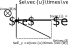
\includegraphics[width=0.5\textwidth]{Chapter_3/Hall_forces}
    \caption{Силы, действующие на носитель заряда в проводящей среде в
электрическом и перпендикулярном ему магнитном полях.}
    \figmark{Hall forces}
\end{figure}
\todo[inline,author=Popo]{Переделать рисунок}

Рассмотрим простейший случай, когда система содержит носители только одного
сорта (например, электроны в большинстве металлов).
Пусть ток течёт по оси~$x$, а магнитное поле направлено по оси $z$
(см. рис.~\figref{Hall forces}).
В таком случае со стороны магнитного поля на движущиеся заряды действует сила
$F_y=-qu_xB_z$, направленная вдоль~$y$, которая должна приводить к
току вдоль оси~$y$. Однако по построению ток течёт по~$x$, поэтому
заряды в среде должны перераспределиться таким образом, чтобы полностью
скомпенсировать эту силу, создав в $y$-направлении электрическое поле
\begin{equation*}
E_y=u_x B_z=\frac{j_x}{nq} B_z,
\end{equation*}
называемое \term{холловским}.
По оси $x$ носители тока будут двигаться так, как если бы
магнитного поля не было, то есть $j_x=\lambda_0 E_x$, $j_y=j_z=0$,
где $\lambda_0 = e^2nb$~--- удельная проводимость среды в отсутствие~$B$.

Получим теперь cвязь между~$\vec{E}$ и~$\vec{j}$ в общем виде.
Ось $z$ по-прежнему направим вдоль магнитного поля~$\vec{B}$, а о
направлении~$\vec{E}$ и~$\vec{j}$ никаких предположений делать не будем.
При течении носителей с постоянной средней скоростью сила Лоренца
\eqref{F-lorentz} будет уравновешена трением со стороны среды \eqref{3.23}:
\begin{equation*}
    q(\vec{E}+\vec{u}\times \vec{B}) - \frac{\vec{u}}{b} =0.
\end{equation*}
С учётом введённых выше обозначений этот баланс сил можно переписать как
\begin{equation}
    \eqmark{ohm-hall}
    \vec{E} = \frac{\vec{j}}{\lambda_0} -
    \frac{1}{nq} \vec{j}\times\vec{B},
\end{equation}
Соотношение \eqref{ohm-hall} можно назвать \important{обобщением закона Ома} при
наличии магнитного поля.

Записывая равенство \eqref{ohm-hall} по-компонентно
\[
E_x = \frac{j_x}{\lambda_0}  -  \frac{j_y B}{nq} ,\qquad
    E_y = \frac{j_y}{\lambda_0} +  \frac{j_xB}{nq} ,\qquad
    E_z = \frac{j_z}{\lambda_0},
\]
можно получить в явном виде
\term{тензор удельного сопротивления}~$\widehat{\rho}$ (обратный к тензору
проводимости):
\begin{equation}
    \vec{E}=\widehat{\rho}\vec{j}= \left(
    \begin{matrix}
        1 & -\beta & {0} \\
        \beta & 1 & {0} \\
        {0} &{0}& 1
    \end{matrix}
    \right)
    \frac{\vec{j}}{\lambda_0},
    \eqmark{3.17}
\end{equation}
где для краткости введено обозначение $\beta = \lambda_0 B / nq  = q b B$.%
\footnote{Физический смысл параметра $\beta$ (называемого иногда
\term{параметром замагниченности})~--- отношение
эффективной длины <<свободного>> пробега частиц~$b/mu$
($b/m$ --- ускорение из-за трения) к ларморовскому радиусу кривизны их
траектории $r_B=mu/qB$.}
Обращением матрицы \eqref{3.17} нетрудно получить тензор проводимости:
\begin{equation}
    \widehat{\lambda}\equiv \widehat{\rho}^{-1}=
    \frac{\lambda_0}{1+\beta^2}\left(
    \begin{matrix}
        {1} & \beta & {0} \\
        -\beta & 1 & {0} \\
        {0} &{0}& 1 \\
    \end{matrix}
    \right).
    \eqmark{3.18}
\end{equation}


Существуют две основных и принципиально различных геометрии для исследования
зависимости проводимости среды от магнитного поля: геометрия \term{мостика
Холла} и геометрия \term{диска Корбино} (см. рис.~\figref{Geometries}).
Рассмотрим их подробнее.

\begin{figure}[h!]
    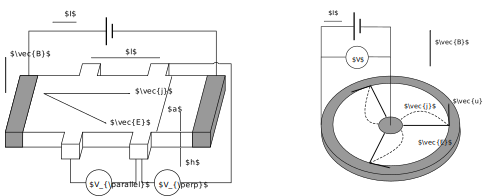
\includegraphics[width=0.9\linewidth]{Chapter_3/2schemes}
    \caption{Две геометрии для исследования влияния магнитного поля на
проводящие свойства: мостик Холла (слева) и диск Корбино (справа).}
    \figmark{Geometries}
\end{figure}

\paragraph{Мостик Холла.}
В~данной геометрии (см. рис.~\figref{Geometries}) ток вынуждают течь по
оси $x$ вдоль плоской пластинки (ширина пластинки $w$, толщина $h$,
длина $l$).
Сила Лоренца, действующая со стороны перпендикулярного
пластинки магнитного поля, прибивает носители заряда к краям образца,
создавая тем самым холловское поле, компенсирующее эту силу.
Поперечное напряжение между краями пластинки
(\term{холловское напряжение}) равно~$V_{\perp}=E_yw$,
где, согласно уравнению \eqref{3.17},
\[
E_y=\rho_{yx}\cdot j_x=j_x B/(nq).
\]
Плотность тока, текущего через образец, равна $j_x=I/wh$, где $I$ ---
полный ток, $wh$ --- поперечное сечение.
Таким образом, для холловского напряжения имеем:
\begin{equation}
    V_{\perp}=\frac{B}{nqh}\cdot I =R_{\rm H}\cdot \frac{B}{h}\cdot I .
    \eqmark{3.19}
\end{equation}
Здесь мы ввели константу
\begin{equation}
    R_{\rm H}= \frac{V_{\perp}h}{IB} = \frac{1}{nq},
    \eqmark{HallConstant}
\end{equation}
которую принято называть \term{постоянной Холла}. В~таблице в приложении даны
постоянные Холла для различных металлов. Для полупроводников постоянные Холла
сильно зависят от наличия малых концентраций примеси и температуры.
Знак постоянной Холла определяется знаком заряда носителей.

Продольная напряжённость равна $E_x = \rho_{xx}\cdot j_x = j_x/\lambda_0$.
Поэтому падение напряжения \important{вдоль} пластинки $V_{\parallel}=E_x l$
определяется просто законом Ома:
\begin{equation}
    V_{\parallel}= I R_x,
    \eqmark{3.20}
\end{equation}
где $R_x = \rho_0 \frac{l}{wh}$ --- омическое сопротивление
образца при протекании тока вдоль~$x$.

Интересно отметить, что несмотря на то, что тензор проводимости \eqref{3.18}
явно зависит от $B$, сопротивление образца в данной геометрии от магнитного поля
\important{не зависит}.

\paragraph{Диск Корбино.}
В~геометрии Корбино (см. рис.~\figref{Geometries}) электрическое поле
направлено по радиусу системы. В~перпендикулярном диску магнитном поле ток
вынужден протекать под углом к электрическому полю, то есть линии тока
представляют собой \important{спирали}. Холловское электрическое
поле при этом не возникает.

Ввиду симметрии системы вклад в полный ток даёт только \important{радиальная}
компонента плотности тока $j_r=\lambda_{r} E_r$. Полный ток равен
$I=j_r \cdot 2\pi r h$, где $r$ --- радиус диска, $h$ --- толщина.
Если система \important{однокомпонентная}, проводимость в радиальном
направлении~$\lambda_r$ соответствует компоненте~$\lambda_{xx}$ тензора
\eqref{3.18}:
\begin{equation}
\lambda_r = \frac{\lambda_0}{1+\beta^2},
\end{equation}
где $\beta = \lambda_0 R_{\rm H} B = q b B$.
Напряжение между центром и краем диска равно
\begin{equation*}
V=\int\limits_{r_1}^{r_2}E_r dr=
\frac{1}{\lambda_r}\int\limits_{r_1}^{r_2} \frac{I}{2\pi r h}dr =
I \frac{\ln \frac{r_2}{r_1}}{\lambda_r 2\pi h}.
\end{equation*}
Величина $R_0 = \dfrac{\ln \frac{r_2}{r_1}}{\lambda_0 2\pi r h}$ есть
сопротивление диска в отсутствие магнитного поля. Поэтому закон Ома
в геометрии Корбино можно записать как
\begin{equation}
    \eqmark{MagnetoSoprot}
    V=I R,\qquad \text{где~}R = R_0 (1+\beta^2).
\end{equation}

Таким образом, в данной геометрии появляется зависимость сопротивления
образца от магнитного поля. Причина этой зависимости --- в геометрии
системы: магнитное поле искривляет линии тока, делая их длиннее.
Такой эффект называют \term{геометрическим магнетосопротивлением}.

\begin{lab:note}
Отметим одну экспериментальную особенность обсуждаемых систем. Измерения в
геометрии мостика Холла представляют собой \important{четырехконтактные}
измерения, то есть два контакта используются для задания тока через образец, а с
двух контактов снимается падение напряжения. Вольтметр обладает
большим сопротивлением (то есть ток через него практически не
течёт), поэтому измеряемое падение напряжения не зависит от свойств
контактов, а определяется только свойствами материала.

Измерения же на диске Корбино проводятся по \important{двухточечной}
схеме, то есть сопротивление образца в ней суммируется с сопротивлениями
контактов. Поэтому исключительно важно создать низкоомные контакты к образцу,
сопротивлением которых можно пренебречь. Для наблюдения этого
магнетосопротивления выбирают систему с большой подвижнотью носителей
(как правило, это полупроводник с низкой эффективной массой электронов,
например InSb).
\end{lab:note}


\paragraph{Магнетосопротивление.}
Зависимость сопротивления образца от величины магнитного поля называют
\term{магнетосопротивлением}.

На примере мостика Холла мы увидели, что для \important{изотропных} веществ с
\important{одним} типом носителя эффект магнетосопротивления
\important{отсутствует}. Для таких веществ зависимость $R(B)$ может проявляться
только в силу геометрических эффектов, как в примере с диском Корбино.

В~общем случае магнетосопротивление материалов может быть отлично от нуля
и в схеме Холла. Это имеет место, если
\important{диагональные} компоненты тензора сопротивления $\widehat{\rho}$
зависят от магнитного поля. Этому могут служить следующие причины:
\begin{enumerate}
    \item Система может быть \important{анизотропной}, то есть в разных
направлениях ($x,y,z$) токопроводящие свойства различны.

\item Система может быть \important{многокомпонентной}. Например, в
полупроводниках часто одновременно существуют электроны и дырки, концентрации
($n_e$ и~$n_p$) и подвижности ($b_e$ и~$b_p$) которых в общем случае
различаются.
% Тогда полный тензор проводимости будет суммой тензоров проводимости двух
% компонент вида \eqref{3.18}. Обращением тензора проводимости в пределе малых
% магнитных полей можно показать, что холловское сопротивление двухкомпонентной
% системы в полупроводнике равно:
% \begin{equation}
%     R_{xy}\equiv \frac{V_{xy}}{I}=\frac{nb_n^2-pb_p^2}{eh(nb_n+pb_p)^2}B
%     \eqmark{3.21}
% \end{equation}

\item Существуют \important{квантовые эффекты} в проводимости, которые приводят
к тому, что \important{подвижность} зависит от магнитного поля. Например, если
проводящий материал является ферромагнетиком, то с ростом поля он
намагничивается, количество доменов уменьшается, а доменные стенки являются
причиной сильного рассеяния, то есть уменьшают подвижность.
\end{enumerate}

\begin{lab:example}
Рассмотрим простейший пример многокомпонентной системы, в которой возникает
эффект магнетосопротивления. Выкладки даже в двух компонентной
системе резко усложняются, поэтому мы приведём лишь схему вывода.

Пусть в среде имеется два типа носителей --- электроны и дырки. Система
уравнений, которым подчиняются носители, по-прежнему представляет собой баланс
сил Лоренца и трения (см. \eqref{ohm-hall}) для каждого компонента в
отдельности:
\begin{equation}
    \eqmark{two-component}
    \begin{aligned}
-e(\vec{E}+\vec{u}_e\times \vec{B}) - \frac{\vec{u}_e}{b_e} &=0,\\
e(\vec{E}+\vec{u}_p\times \vec{B}) - \frac{\vec{u}_p}{b_p} &=0.
\end{aligned}
\end{equation}
Повторяя вывод \eqref{3.18} для каждого сорта носителей отдельно, можно
получить связь напряжённостью поля и плотностями тока этих носителей:
\begin{equation}
    \vec{j}_e = -en_e \vec{u}_e = \widehat{\lambda}_e \vec{E},\qquad
    \vec{j}_p = en_p \vec{u}_p = \widehat{\lambda}_p \vec{E}.
\end{equation}
Тензоры проводимости будут определяться \eqref{3.18}, где нужно проставить
индексы, соответствующие сорту носителя.
Полная плотность тока есть
\[
\vec{j} = \vec{j}_e + \vec{j}_p = \widehat{\lambda}_e \vec{E} +
\widehat{\lambda}_p \vec{E},
\]
поэтому тензор проводимости среды равен
\[
\widehat{\lambda} = \widehat{\lambda}_e + \widehat{\lambda}_p.
\]
Обращая $\widehat{\lambda}$, можно получить тензор удельного сопротивления:
$\widehat{\rho}=
\left(\widehat{\rho}_e^{-1}+\widehat{\rho}_i^{-1}\right)^{-1}$.

Для справки приведём ответы.
% Диагональная компонента тензора сопротивления,
% отвечающая за эффект \important{магнетосопротивления}, равна
% \[
% \rho_{xx} = \frac{\lambda_p (1+\beta_e^2) + \lambda_e (1+\beta_p^2)}%
% {(\beta_p\lambda_e-\beta_e\lambda_p)^2 + (\lambda_e+\lambda_p)^2}.
% \]
% <<Косая>> компонента тензора, отвечающая \important{эффекту Холла}:
% \[
% \rho_{yx} = \frac{\beta_p\lambda_p (1+\beta_e^2) -
% \beta_e\lambda_e (1+\beta_p^2)}%
% {(\beta_p\lambda_e-\beta_e\lambda_p)^2 + (\lambda_e+\lambda_p)^2}.
% \]
В опыте с мостиком Холла продольная компонента электрического поля равна
\[
E_x = \frac{(\beta_p^2+1) \lambda_e+ (\beta_e^2 +1)\lambda_p}%
{ (\beta_e \lambda_p-\beta_p \lambda_e)^2 + (\lambda_e+\lambda_p)^2}
j.
\]
Видно, что удельное сопротивление в этом направлении сложным образом
зависит от~$B$, то есть имеет место эффект \important{магнетосопротивления}.
Однако в слабых полях ($\beta \ll 1$) эффект довольно мал (поправка
квадратична по~$\beta$).

Поперечная компонента (\important{холловское поле}) также имеет сложную
зависимость от магнитного поля:
\[
E_y = \frac{\beta_e\beta_p(\beta_e\lambda_p-\beta_p\lambda_e)+
    \beta_p \lambda_p -\beta_e \lambda_e}%
{(\beta_e \lambda_p - \beta_p \lambda_e)^2 + (\lambda_e+\lambda_p)^2} j.
\]

Отсюда можно получить постоянную Холла в полупроводнике в пределе малого
магнитного поля ($\beta \ll 1$):
\begin{equation}
    \eqmark{3.21}
    R_{\rm H} = \frac{b_p^2 n_p - b_e^2 n_e}%
{e(b_en_e+b_pn_p)^2}.
\end{equation}
\end{lab:example}


\begin{lab:literature}
    \item{ \textit{Сивухин Д.В.} Общий курс физики.~--- T.~III.
Электричество.~---
М.: Наука, 1983. \S\S~86, 95, 98, 100.}
    \item{ \textit{Кингсеп А.С., Локшин Г.Р., Ольхов О.А.} Основы физики.
Т.~1.~--- М.: Физматлит, 2001. \S\S~8.1--8.3.}
\end{lab:literature}


\todo[inline,author=Popov,color=cyan]{Перенести в описание работы --->}
Измерение заряда капель производится путём исследования их движения в
электрическом поле. В~расположенный горизонтально плоский конденсатор через
отверстие в верхней пластине впрыскиваются мелкие капельки масла, получаемые с
помощью специального распылителя. На пластины конденсатора подаётся постоянное
напряжение (порядка нескольких киловольт). В~ходе опыта это напряжение можно
изменять. При распылении капельки масла вследствие трения о воздух приобретают
случайный по величине и знаку электрический заряд. Попадая в конденсатор,
капельки масла движутся в воздухе, опускаясь под действием силы тяжести или
поднимаясь под действием электрического поля. Время~$t_0$ опускания капли и
время её обратного подъёма~$t$ легко измерить с необходимой точностью.
Оказывается, что именно к измерению этих двух интервалов времени и сводится
измерение заряда капли.

Разумеется, дискретность заряда разных капель и, следовательно, величина
элементарного заряда, то есть заряд электрона, могут быть обнаружены только в
том случае, если абсолютная ошибка в измерении заряда капли будет существенно
меньше самого элементарного заряда. В~опытах Милликена необходимая точность
вполне может быть обеспечена в условиях лабораторного практикума.
\todo[inline,color=cyan]{<---}

\todo[inline,author=Popov,color=cyan]{Убрать в описание работы --->}
\paragraph{Метод магнитной фокусировки для измерения $e/m$.}
Найдём расстояние~$L$, которое проходит электрон в направлении вдоль поля за
один
оборот (шаг винтовой линии). Время одного оборота~$T_c$,
называемое \term{циклотронным периодом}, равно
$T_c= \frac{2\pi R}{v_{\perp}}$. Заменяя $R/v_{\perp}$ c помощью \eqref{3.4},
найдём
\begin{equation}
    \eqmark{3.5}
    T_c =\frac{2\pi m}{eB}.
\end{equation}

За это время электрон проходит вдоль магнитного поля расстояние
\begin{equation}
    \eqmark{3.6}
    L = v_{\parallel}T_c =\frac{2\pi v\cos\alpha}{(e/m)B}.
\end{equation}

Если углы невелики $\alpha \ll 1$, то $\cos\alpha \approx 1$ и
\begin{equation}
    \eqmark{3.7}
    L \approx \frac{2\pi v}{(e/m)B}.
\end{equation}
Таким образом, при малых углах расстояние~$L$ не зависит от~$\alpha$, так
что все электроны, вышедшие из одной точки, после одного оборота вновь соберутся
в одной точке~--- сфокусируются. Как следует из \eqref{3.7}, индукция поля~$B$,
при которой точка фокусировки отстоит от точки вылета на расстоянии~$L$, зависит
от величины~$e/m$~--- удельного заряда электрона.

Скорость движения электрона определяется разность потенциалов~$V$,
пройденную им до попадания в магнитное поле:
\begin{equation*}
  \frac{mv^2}{2}=eV,
\end{equation*}
откуда
\begin{equation}
  \eqmark{3.3}
  v=\sqrt{\frac{2eV}{m}}.
%   = 6\cdot10^5\sqrt{V}~\frac{m}{c}.
\end{equation}

Обозначим через~$B_{ф}$ индукцию магнитного поля, при которой наступает
фокусировка.
Используя \eqref{3.3} и \eqref{3.7}, выразим удельный заряд электрона~$e/m$
через~$B_{ф}$:
\begin{equation}
\eqmark{3.8}
\frac{e}{m}=\frac{8\pi^2 V}{L^2B_{ф}^2}.
\end{equation}
Эта формула положена в основу экспериментального измерения удельного заряда
электрона по \important{методу магнитной фокусировки}.
\todo[inline,color=cyan]{<---}

\todo[inline,author=Popov,color=cyan]{Убрать в описание работы --->}
В~так называемом {\important{методе магнетрона}} отношение~$e/m$ измеряется на
основе исследования движения электрона в скрещенных электрическом и магнитном
полях, перпендикулярных друг другу. Название метода связано с тем, что такая
конфигурация электрического и магнитного полей реализуется в магнетронах~---
генераторах электромагнитных колебаний
сверхвысоких частот.

\begin{figure}[h!]
    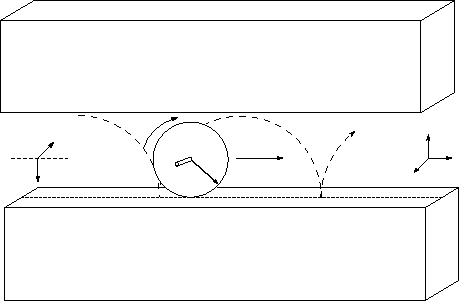
\includegraphics[width=\textwidth]{v3_3}
    \caption{Движение заряда в скрещенных полях}
    \figmark{Crossed fields}
\end{figure}
\todo[inline,author=Popov]{Рисунок странный. Что там по центру? Надо бы
нарисовать другой}

Для уяснения идеи метода магнетрона, рассмотрим вначале движение заряда в
<<плоском магнетроне>>, который можно
представить себе в виде плоского конденсатора, помещённого в магнитное поле так,
что $\vec{E}\perp\vec{B}$ (рис.~\figref{Crossed fields}). При этом отрицательная
пластина конденсатора играет роль катода, положительная соответственно анода.
Если бы магнитного поля не было, то все электроны, вылетевшие без начальной
скорости из катода такого плоского диода, попадали бы на анод. При наличии
магнитного поля траектории электронов искривляются, вследствие чего при
достаточно большом магнитном поле ни один электрон не достигнет анода. Для
заданного напряжения между катодом и анодом существует некоторое критическое
значение магнитной индукции~$B_\text{кр}$, при котором траектории касаются
поверхности анода. Если~$B<B_\text{кр}$, то все электроны достигают анода и ток
через магнетрон имеет то же значение, что и без магнитного поля. Если же
$B>B_\text{кр}$, то электроны не достигают анода и ток через лампу равен нулю.

Рассчитаем это критическое значение индукции магнитного поля. Уравнения движения
электрона в нашем случае имеет вид
\begin{equation}
    \eqmark{3.9}
    m\frac{dv_x}{dt}=ev_y B,
\end{equation}
\begin{equation}
    \eqmark{3.10}
    m\frac{dv_y}{dt}=eE-ev_x B
\end{equation}
при начальных условиях $x(0)=y(0)=0$, $v_x(0)=v_y(0)=0$.

Непосредственной подстановкой несложно убедиться в том, что решением системы
дифференциальных уравнений с заданными
начальными условиями является уравнение циклоиды (в параметрической форме):
\begin{equation}
    \eqmark{3.11}
    x = vt - R\sin\omega t,\qquad y = R(1-\cos\omega t),
\end{equation}
где $ v=E/B$, $R=v/\omega=Em/(eB^2)$.

Касание анода происходит при $2R=d$ ($d$~--- расстояние между анодом и катодом).
Этому значению соответствует
критическое поле
\begin{equation}
    B_\text{кр}=\frac{\sqrt{2V}}{d\sqrt{e/m}}.
    \eqmark{3.12}
\end{equation}
Из последней формулы находим удельный заряд:
\begin{equation}
    \eqmark{3.13}
    \frac{e}{m}=\frac{2V}{d^2B_\text{кр}^2}.
\end{equation}
\todo[inline,author=Popov]{Убрать детали в описание работы. Во введении ---
    только общие соотношения}

Эта формула позволяет вычислить~$e/m$, если при заданном значении напряжения на
аноде~$V$ найти такое значение
магнитного поля, при превышении которого ток в магнетроне отсутствует.
\todo[inline,color=cyan]{<---}

\todo[inline,author=Popov,color=cyan]{Убрать в описание работы и там дополнить
--->}
Теперь задача о распределении потенциала становится однозначной и приводит к
решению
\begin{equation*}
    j=\frac{4\varepsilon_0}{9x^2}\sqrt{\frac{2e}{m}}\varphi^{3/2}.
\end{equation*}
\todo[inline,author=Popov]{Убрать детали в описание работы,
во введении --- только общие законы}

Так как $\varphi(d)=V$, где~$d$~--- расстояние между электродами, то для
зависимости тока от напряжения получаем
\begin{equation*}
    I=\frac{4\varepsilon_0 S}{9d^2}\sqrt{\frac{2e}{m}}V^{3/2},
\end{equation*}
где~$S$~--- площадь катода. Мы получили зависимость тока через плоский диод от
приложенного к нему напряжения, известную как <<закон трёх вторых>> для плоского
диода. Оказывается, что не только для плоского вакуумного диода, а и для
вакуумного диода с электродами любой другой геометрии ток подчиняется <<закону
степени трёх вторых>>.

Полученная формула подсказывает процедуру измерения удельного заряда электрона.
Для этого достаточно по
результатам эксперимента построить график зависимости тока от напряжения в
степени трёх вторых, который должен
представлять собой прямую линию, проходящую через начало координат. Угол наклона
этой прямой линии пропорционален (с известным коэффициентом) квадратному корню
из~$e/m$~--- искомой величины удельного заряда электрона.
\todo[inline,color=cyan]{<---}
